%==============================================================================
% Multi-Agent Byzantine Fault Tolerant Consensus System - LaTeX Figures
% For OverLeaf - Use with XeLaTeX or LuaLaTeX
% Required packages: pgfplots, amsmath, amssymb, booktabs, geometry
%==============================================================================

\documentclass{article}
\usepackage{pgfplots}
\usepackage{pgfplotstable}
\usepackage{amsmath}
\usepackage{amssymb}
\usepackage{booktabs}
\usepackage{geometry}
\usepackage{caption}
\usepackage{subcaption}

\geometry{a4paper, margin=0.8in}

% Color definitions
\definecolor{cfo}{RGB}{46,134,171}
\definecolor{pbft}{RGB}{161,59,114}
\definecolor{krum}{RGB}{241,143,1}
\definecolor{trimmedmean}{RGB}{199,62,29}
\definecolor{median}{RGB}{106,153,78}
\definecolor{aggregation}{RGB}{70,153,206}
\definecolor{trust}{RGB}{100,100,100}

% PGFPlots settings
\pgfplotsset{
    width=10cm,
    height=6cm,
    compat=1.18,
    tick label style={font=\fontsize{9}{11}\selectfont},
    label style={font=\fontsize{10}{12}\selectfont},
    legend style={font=\fontsize{8}{10}\selectfont},
    title style={font=\fontsize{11}{13}\selectfont},
}

\begin{document}

%==============================================================================
% FIGURE 1: Comparison with Traditional BFT Consensus (Combined Dual-Axis)
%==============================================================================
\begin{figure}[htbp]
\centering
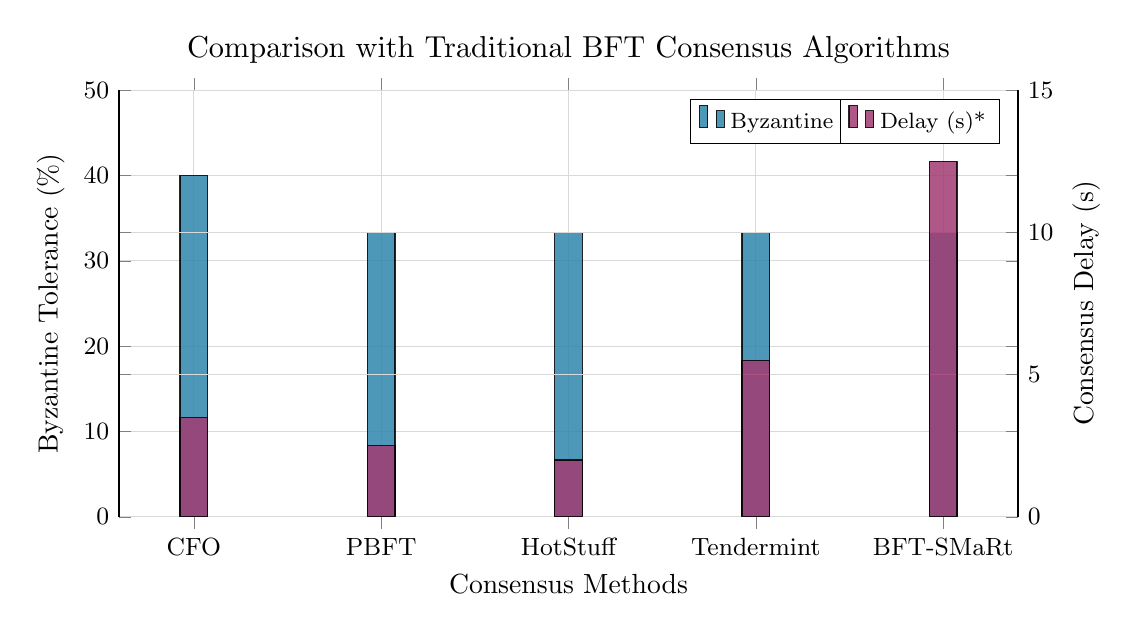
\begin{tikzpicture}
\begin{axis}[
    width=13cm,
    height=7cm,
    ybar=0.32,
    bar width=10pt,
    ymin=0, ymax=50,
    ylabel={Byzantine Tolerance (\%)},
    xlabel={Consensus Methods},
    title={Comparison with Traditional BFT Consensus Algorithms},
    grid=major,
    major grid style={gray!30},
    symbolic x coords={CFO, PBFT, HotStuff, Tendermint, BFT-SMaRt},
    xtick=data,
]

\addplot[fill=cfo, draw=black, opacity=0.85] coordinates {
    (CFO, 40)
    (PBFT, 33.3)
    (HotStuff, 33.3)
    (Tendermint, 33.3)
    (BFT-SMaRt, 33.3)
};
\addlegendentry{Byzantine Tolerance (\%)}

\end{axis}
%
\begin{axis}[
    width=13cm,
    height=7cm,
    ybar=0.32,
    bar width=10pt,
    ymin=0, ymax=15,
    ylabel near ticks,
    yticklabel pos=right,
    ylabel={Consensus Delay (s)},
    grid=major,
    major grid style={gray!30},
    symbolic x coords={CFO, PBFT, HotStuff, Tendermint, BFT-SMaRt},
    xtick=data,
    hide x axis,
]

\addplot[fill=pbft, draw=black, opacity=0.85] coordinates {
    (CFO, 3.5)
    (PBFT, 2.5)
    (HotStuff, 2)
    (Tendermint, 5.5)
    (BFT-SMaRt, 12.5)
};
\addlegendentry{Delay (s)*}

\end{axis}
\end{tikzpicture}
\\
{\fontsize{8}{10}\selectfont *CFO: $\sim$3.5s consensus (excluding 60-90s for 30 LLM API calls) | CFO achieves 40\% Byzantine tolerance vs 33.3\% limit}
\caption{Comparison with Traditional BFT Consensus Algorithms}
\label{fig:bft_comparison}
\end{figure}

%==============================================================================
% FIGURE 2: Comparison with Federated Learning Byzantine Defense Methods
%==============================================================================
\begin{figure}[htbp]
\begin{minipage}{0.48\textwidth}
\begin{tikzpicture}
\begin{axis}[
    xbar=0.5,
    bar width=10pt,
    symbolic y coords={CFO, Krum, Trimmed Mean, Median, Multi-Krum, Bulyan},
    ytick=data,
    xmin=75, xmax=100,
    xlabel={Accuracy (\%)},
    title={(a) Prediction Accuracy},
    grid=major,
]

\addplot[fill=cfo, draw=black] coordinates {(94.08, CFO)};
\addplot[fill=krum, draw=black] coordinates {(85, Krum)};
\addplot[fill=trimmedmean, draw=black] coordinates {(80, Trimmed Mean)};
\addplot[fill=median, draw=black] coordinates {(80, Median)};
\addplot[fill=aggregation, draw=black] coordinates {(90, Multi-Krum)};
\addplot[fill=pbft, draw=black] coordinates {(88, Bulyan)};

\end{axis}
\end{tikzpicture}
\end{minipage}
\hfill
\begin{minipage}{0.48\textwidth}
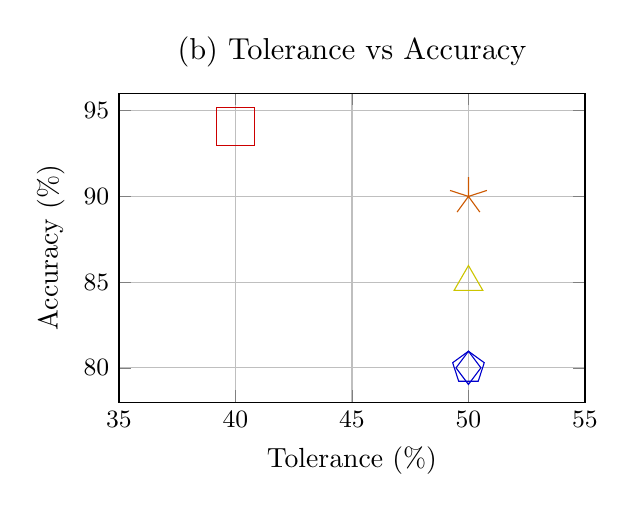
\begin{tikzpicture}
\begin{axis}[
    width=7.5cm,
    height=5.5cm,
    scatter,
    xmin=35, xmax=55,
    ymin=78, ymax=96,
    xlabel={Tolerance (\%)},
    ylabel={Accuracy (\%)},
    title={(b) Tolerance vs Accuracy},
    grid=major,
]

\addplot[scatter,only marks,mark=square,mark size=7pt,color=cfo] coordinates {(40, 94.08)};
\addplot[scatter,only marks,mark=triangle,mark size=6pt,color=krum] coordinates {(50, 85)};
\addplot[scatter,only marks,mark=diamond,mark size=6pt,color=trimmedmean] coordinates {(50, 80)};
\addplot[scatter,only marks,mark=pentagon,mark size=6pt,color=median] coordinates {(50, 80)};
\addplot[scatter,only marks,mark=star,mark size=7pt,color=aggregation] coordinates {(50, 90)};
\addplot[scatter,only marks,mark=plus,mark size=7pt,color=pbft] coordinates {(50, 88)};

\end{axis}
\end{tikzpicture}
\end{minipage}
\caption{Comparison with Federated Learning Byzantine Defense Methods}
\label{fig:federated_comparison}
\end{figure}

%==============================================================================
% FIGURE 3: Comparison with Multi-Agent Consensus Methods (Combined)
%==============================================================================
\begin{figure}[htbp]
\centering
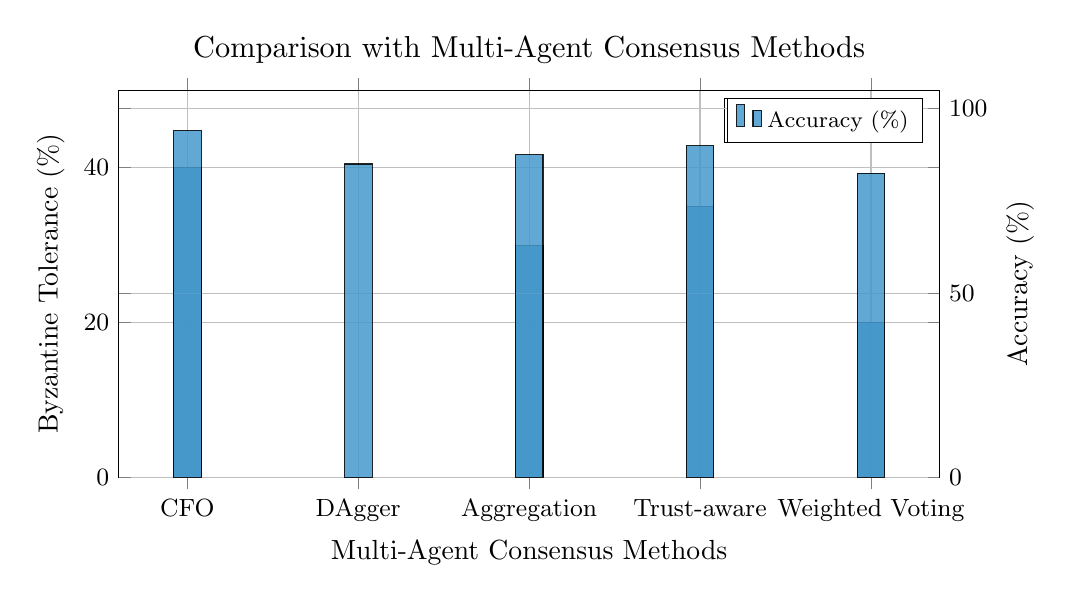
\begin{tikzpicture}
\begin{axis}[
    width=12cm,
    height=6.5cm,
    ybar=0.32,
    bar width=10pt,
    ymin=0, ymax=50,
    ylabel={Byzantine Tolerance (\%)},
    xlabel={Multi-Agent Consensus Methods},
    title={Comparison with Multi-Agent Consensus Methods},
    grid=major,
    symbolic x coords={CFO, DAgger, Aggregation, Trust-aware, Weighted Voting},
    xtick=data,
]

\addplot[fill=cfo, draw=black, opacity=0.85] coordinates {
    (CFO, 40)
    (DAgger, 0)
    (Aggregation, 30)
    (Trust-aware, 35)
    (Weighted Voting, 20)
};
\addlegendentry{Tolerance (\%)}

\end{axis}
%
\begin{axis}[
    width=12cm,
    height=6.5cm,
    ybar=0.32,
    bar width=10pt,
    ymin=0, ymax=105,
    ylabel near ticks,
    yticklabel pos=right,
    ylabel={Accuracy (\%)},
    grid=major,
    symbolic x coords={CFO, DAgger, Aggregation, Trust-aware, Weighted Voting},
    xtick=data,
    hide x axis,
]

\addplot[fill=aggregation, draw=black, opacity=0.85] coordinates {
    (CFO, 94.08)
    (DAgger, 85)
    (Aggregation, 87.5)
    (Trust-aware, 90)
    (Weighted Voting, 82.5)
};
\addlegendentry{Accuracy (\%)}

\end{axis}
\end{tikzpicture}
\\
{\fontsize{8}{10}\selectfont *CFO: 40\% tolerance + 94.08\% accuracy - both highest among all methods}
\caption{Comparison with Multi-Agent Consensus Methods}
\label{fig:multi_agent_comparison}
\end{figure}

%==============================================================================
% FIGURE 4: Byzantine Tolerance vs Accuracy Trend
%==============================================================================
\begin{figure}[htbp]
\centering
\begin{tikzpicture}
\begin{axis}[
    width=11cm,
    height=7cm,
    xmin=0, xmax=42,
    ymin=70, ymax=100,
    xlabel={Byzantine Node Ratio (\%)},
    ylabel={Average Accuracy (\%)},
    title={Relationship between Byzantine Tolerance and Prediction Accuracy},
    grid=major,
    major grid style={gray!30},
    legend pos=lower left,
]

\addplot[color=cfo, line width=2pt, mark=square, mark size=6pt] coordinates {
    (0, 97.62) (10, 95.88) (20, 94.23) (30, 92.47) (40, 91.35)
};
\addlegendentry{CFO (ours)}

\addplot[color=krum, line width=1.5pt, dashed, mark=triangle, mark size=5pt] coordinates {
    (0, 95) (10, 92) (20, 89) (30, 86) (40, 83)
};
\addlegendentry{Krum}

\addplot[color=trimmedmean, line width=1.5pt, dashed, mark=diamond, mark size=5pt] coordinates {
    (0, 92) (10, 88) (20, 84) (30, 80) (40, 76)
};
\addlegendentry{Trimmed Mean}

\addplot[color=median, line width=1.5pt, dashed, mark=pentagon, mark size=5pt] coordinates {
    (0, 90) (10, 86) (20, 82) (30, 78) (40, 74)
};
\addlegendentry{Median}

\end{axis}
\end{tikzpicture}
\\
{\fontsize{8}{10}\selectfont *CFO maintains high accuracy (91.35\%) even at 40\% Byzantine ratio, far exceeding traditional 33.3\% limit}
\caption{Byzantine Tolerance vs Prediction Accuracy Trend}
\label{fig:tolerance_accuracy_trend}
\end{figure}

%==============================================================================
% SUMMARY TABLE
%==============================================================================
\begin{table}[htbp]
\centering
\caption{Detailed Comparison with Existing Methods}
\label{tab:comparison}
\begin{subtable}{0.48\textwidth}
\centering
\caption{BFT Consensus Methods}
\begin{tabular}{|l|c|c|c|c|}
\toprule
Method & Tol. & Acc. & Delay & Comm. \\
\midrule
CFO & \textbf{40\%} & \textbf{94.1\%} & 3.5s* & $O(n^2)$ \\
PBFT & 33.3\% & - & 2-5s & $O(n^2)$ \\
HotStuff & 33.3\% & - & 1-3s & $O(n)$ \\
Tendermint & 33.3\% & - & 1-10s & $O(n^2)$ \\
\bottomrule
\end{tabular}
\end{subtable}
\hfill
\begin{subtable}{0.48\textwidth}
\caption{Federated Defense Methods}
\begin{tabular}{|l|c|c|c|c|}
\toprule
Method & Tol. & Acc. & Delay & Comm. \\
\midrule
CFO & \textbf{40\%} & \textbf{94.1\%} & 3.5s* & $O(n^2)$ \\
Krum & 50\% & 85\% & - & Low \\
Trimmed Mean & 50\% & 80\% & - & Low \\
Median & 50\% & 80\% & - & Low \\
Multi-Krum & 50\% & 90\% & - & Med \\
\bottomrule
\end{tabular}
\end{subtable}
\\
{\fontsize{8}{9}\selectfont *CFO: 3.5s consensus algorithm time (excluding 60-90s LLM API calls)}
\end{table}

\end{document}
